\documentclass[fleqn, a4paper, 12pt, twoside]{article}
\usepackage{exsheets}
\usepackage{amsmath, amssymb, amsthm} %standard AMS packages
\usepackage{marginnote} %marginnotes
\usepackage{gensymb} %miscellaneous symbols
\usepackage{commath} %differential symbols
\usepackage{xcolor} %colours
\usepackage{cancel} %cancelling terms
\usepackage{siunitx} %formatting units
\usepackage{tikz, pgfplots} %diagrams
	\usetikzlibrary{calc, hobby, patterns, intersections}
\usepackage{graphicx} %inserting graphics
\usepackage{hyperref} %hyperlinks
\usepackage{datetime} %date and time
\usepackage{ulem} %underline for \emph{}
\usepackage{xfrac, lmodern} %inline fractions
\usepackage{enumerate} %numbered lists
\usepackage{float} %inserting floats
\usepackage{tabularx}

\newcommand\numberthis{\addtocounter{equation}{1}\tag{\theequation}} %adds numbers to specific equations in non-numbered list of equations

\newcommand{\AxisRotator}[1][rotate=0]{
	\tikz [x=0.25cm,y=0.60cm,line width=.2ex,-stealth,#1] \draw (0,0) arc (-150:150:1 and 1);%
} %rotation symbols on axes

\theoremstyle{definition}
\newtheorem{example}{Example}
\newtheorem{definition}{Definition}

\theoremstyle{theorem}
\newtheorem{theorem}{Theorem}

\newcommand{\curl}{\mathrm{curl\,}}

\makeatletter
\@addtoreset{section}{part} %resets section numbers in new part
\makeatother

\newcommand\blfootnote[1]{%
	\begingroup
	\renewcommand\thefootnote{}\footnote{#1}%
	\addtocounter{footnote}{-1}%
	\endgroup
}

\SetupExSheets{solution/print = true} %prints all solutions by default
%opening
\title{Differential and Integral Calculus}
\author{Aakash Jog}
\date{2014-15}

\begin{document}

\maketitle
%\setlength{\mathindent}{0pt}

\blfootnote
{	
	\begin{figure}[H]
		
\includegraphics[height = 12pt]{cc.eps}
		\includegraphics[height = 12pt]{by.eps}
		\includegraphics[height = 12pt]{nc.eps}
		\includegraphics[height = 12pt]{sa.eps}
	\end{figure}
	This work is licensed under the Creative Commons Attribution-NonCommercial-ShareAlike 4.0 International License. To view a copy of this license, visit \url{http://creativecommons.org/licenses/by-nc-sa/4.0/}.
} %CC-BY-NC-SA licencse

\tableofcontents

\newpage
\section{Lecturer Information}

\textbf{Dr. Yakov Yakubov}\\
~\\
Office: Schreiber 233\\
Telephone: {\href{tel:+97236405357}{+972 3-640-5357}\\
E-mail: \href{mailto:yakubov@post.tau.ac.il}{yakubov@post.tau.ac.il}\\

\section{Required Reading}

Protter and Morrey: \textit{A first Course in Real Analysis}, UTM Series, Springer-Verlag, 1991

\section{Additional Reading}

Thomas and Finney, \textit{Calculus and Analytic Geometry}, 9th edition, Addison-Wesley, 1996

\newpage
\part{Sequences and Series}

\section{Sequences}

\begin{definition}[Sequence]
	A sequence of real numbers is a set of numbers which are written in some order. There are infinitely many terms in a sequence. It is denoted by $\{a_n\}_{n = 1}^{\infty}$ or $\{a_n\}$.
\end{definition}

\begin{example}
	$1, \dfrac{1}{2}, \dfrac{1}{3}, \dots$ is called the harmonic sequence.
	\begin{equation*}
		a_n = \dfrac{1}{n}
	\end{equation*}
\end{example}

\begin{example}
	$1, -\dfrac{1}{2}, \dfrac{1}{3}, \dots$ is called the alternating harmonic sequence.
	\begin{equation*}
		a_n = (-1)^{n + 1} \dfrac{1}{n}
	\end{equation*}
\end{example}

\begin{example}
	$\dfrac{1}{2}, \dfrac{2}{3}, \dfrac{3}{4}, \dots$
	\begin{equation*}
		a_n = \dfrac{n}{n + 1}
	\end{equation*}
\end{example}

\begin{example}
	$\dfrac{2}{3}, \dfrac{3}{9}, \dfrac{4}{27}, \dots$
	\begin{align*}
		a_n = \dfrac{n + 1}{3^n}
	\end{align*}
\end{example}

\begin{example}
	The Fibonacci sequence is given by
	\begin{equation*}
		f_n =
			\begin{cases}
				1 &;\quad n = 1, 2\\
				f_{n - 1} + f_{n - 2} &;\quad n \geq 3\\
			\end{cases}
	\end{equation*}
\end{example}

\begin{example}
	A geometric sequence is given by
	\begin{equation*}
		a_n = a_1 q^{n - 1}
	\end{equation*}
	where $q$ is called the common ratio.
\end{example}

\begin{example}
	A geometric sequence is given by
	\begin{equation*}
		a_n = a_1 + d(n - 1)
	\end{equation*}
	where $d$ is called the common difference.
\end{example}

\begin{definition}[Equal sequences]
	Two sequences $\{a_n\}$ and $\{b_n\}$ are said to be equal if $a_n = b_n$, $\forall n \in \mathbb{N}$.
\end{definition}

\begin{definition}[Sequences bounded from above]
	$\{a_n\}$ is said to be bounded from above if $\exists M \in \mathbb{R}$, s.t. $a_n \leq M$, $\forall n \in \mathbb{N}$.
	Each such $M$ is called an upper bound of $\{a_n\}$.
\end{definition}

\begin{definition}[Sequences bounded from below]
	$\{a_n\}$ is said to be bounded from below if $\exists m \in \mathbb{R}$, s.t. $a_n \geq M$, $\forall n \in \mathbb{N}$.
	Each such $M$ is called an lower bound of $\{a_n\}$.
\end{definition}

\begin{definition}
	$\{a_n\}$ is said to be bounded if it is bounded from below and bounded from above.
\end{definition}

\begin{example}
	The sequence $a_n = n^2 + 2$ is not bounded from above but is bounded from below, by all $m \leq 3$.
\end{example}

\begin{example}
	$\left\{ \dfrac{2n - 1}{3n} \right\}$ is bounded.
	\begin{equation*}
		m = 0 \leq \dfrac{2n - 1}{3n} \leq \dfrac{2n}{3n} = \dfrac{2}{3} = M
	\end{equation*}
\end{example}

\begin{definition}[Monotonic increasing sequence]
	A sequence $\{a_n\}$ is called monotonic increasing if $\exists n_0 \in \mathbb{N}$, s.t. $a_n \leq a_{n + 1}$, $\forall n \geq n_0$.
\end{definition}

\begin{definition}[Monotonic decreasing sequence]
	A sequence $\{a_n\}$ is called monotonic decreasing if $\exists n_0 \in \mathbb{N}$, s.t. $a_n \geq a_{n + 1}$, $\forall n \geq n_0$.
\end{definition}

\begin{definition}[Strongly increasing sequence]
	A sequence $\{a_n\}$ is called monotonic increasing if $\exists n_0 \in \mathbb{N}$, s.t. $a_n < a_{n + 1}$, $\forall n \geq n_0$.
\end{definition}

\begin{definition}[Strongly decreasing sequence]
	A sequence $\{a_n\}$ is called monotonic decreasing if $\exists n_0 \in \mathbb{N}$, s.t. $a_n > a_{n + 1}$, $\forall n \geq n_0$.
\end{definition}

\begin{example}
	The sequence $\left\{ \dfrac{n^2}{2^n} \right\}$ is strongly decreasing.
	However, this is not evident by observing the first few terms.
	$\dfrac{1}{2}, 1, \dfrac{9}{8}, 1, \dfrac{25}{32}, \dots$
	\begin{align*}
		a_n &> a_{n + 1}\\
		\iff \dfrac{n^2}{2^n} &> \dfrac{(n + 1)^2}{2^{n + 1}}\\
		\iff 2 n^2 &> (n + 1)^2\\
		\iff \sqrt{2} n &> n + 1\\
		\iff n(\sqrt{2} - 1) &> 1\\
		\iff n &> \dfrac{1}{\sqrt{2} - 1}\\
		\iff n &> 3
	\end{align*}
\end{example}

\begin{question}
	Is $a_n = (-1)^n$ monotonic?
\end{question}

\begin{solution}[print]
	The sequence $-1, 1, -1, 1, \dots$ is not monotonic.
\end{solution}

\subsection{Limit of a Sequence}

\begin{definition}
	Let $\{a_n\}$ be a given sequence.
	A number $L$ is said to be the limit of the sequence if $\forall \varepsilon > 0$, $\exists n_0 \in \mathbb{N}$, s.t. $|a_n - L| < \varepsilon$, $\forall n \geq n_0$.
	That is, there are infinitely many terms inside the interval and a finite number of terms outside it.
\end{definition}

\begin{example}
	The sequence $\{\dfrac{1}{n}\}$ tends to 0, i.e. for any open interval $(-\varepsilon, \varepsilon)$, there are finite number of terms of the sequence outside the interval, and therefore there are infinitely many terms inside the interval.
\end{example}

\begin{question}
	Prove
	\begin{equation*}
		\lim\limits_{n \to \infty} \dfrac{n + 2}{2n - 1} = \dfrac{1}{2}
	\end{equation*}
\end{question}

\begin{solution}
	$\forall \varepsilon > 0$, $\exists n_0 \in \mathbb{N}$
\end{solution}

\begin{question}
	Prove that 2 is not a limit of $\left\{ \dfrac{3n + 1}{n} \right\}$.
\end{question}

\begin{solution}
	If possible, let 
	\begin{align*}
		\lim\limits_{n \to \infty} \dfrac{3n + 1}{n} = 2
	\end{align*}
	Then, $\forall \varepsilon > 0$, $\exists n_0 \in \mathbb{N}$, s.t. $\left| \dfrac{3n + 1}{n} - 2 \right| < \varepsilon$, $\forall n \geq n_0$.
	However,
	\begin{equation*}
		\left| \dfrac{3n + 1}{n} - 2 \right| = 1 + \dfrac{1}{n} > 1
	\end{equation*}
	This is a contradiction for $\varepsilon = \dfrac{1}{2}$.
	Therefore, 2 is not a limit.
\end{solution}

\begin{theorem}
	If a sequence $\{a_n\}$ has a limit $L$ then the limit is unique.
	\label{uniquness of a limit}
\end{theorem}

\begin{proof}
	If possible let there exist two limits $L_1$ and $L_2$.
	Therefore, $\forall \varepsilon > 0$, there exist a finite number of terms in the interval $(L_1 - \varepsilon, L_1 + \varepsilon)$.
	Therefore, there exist a finite number of terms in the interval $(L_2 - \varepsilon, L_2 + \varepsilon)$.
	This contradicts the definition of a limit.
	Therefore, the limit is unique.
\end{proof}

\begin{theorem}
	If a sequence $\{a_n\}$ has limit $L$, then the sequence is bounded.
	\label{existence of limit implies boundedness}
\end{theorem}

\begin{theorem}
	Let
	\begin{align*}
		\lim\limits_{n \to \infty} a_n &= a\\
		\lim\limits_{n \to \infty} b_n &= b
	\end{align*}
	and let $c$ be a constant.
	Then,
	\begin{align*}
		\lim c &= c\\
		\lim (c a_n) &= c \lim a_n\\
		\lim (a_n \pm b_n) &= \lim a_n \pm \lim b_n\\
		\lim (a_n b_n) &= \lim a_n \lim b_n\\
		\lim (\dfrac{a_n}{b_n}) &= \dfrac{\lim a_n}{\lim b_n} \quad (\textnormal{ if } \lim b \neq 0)
	\end{align*}
	\label{limit arithmetic}
\end{theorem}

\begin{theorem}
	Let $\{b_n\}$ be bounded and let $\lim a_n = 0$. Then,
	\begin{equation*}
		\lim (a_n b_n) = 0
	\end{equation*}
\end{theorem}

\begin{theorem}[Sandwich Theorem]
	Let $\{a_n\}$, $\{b_n\}$, $\{c_n\}$ be three sequences. If
	\begin{equation*}
		\lim a_n = \lim b_n = L
	\end{equation*}
	and $\exists n_0 \in \mathbb{N}$, s.t. $\forall n \geq n_0$, $a_n \leq b_n \leq c_n$.
	Then,
	\begin{equation*}
		\lim b_n = L
	\end{equation*}
	\label{sandwich theorem}
\end{theorem}

\begin{question}
	Calculate $\lim\limits_{n \to \infty} \sqrt[n]{2^n + 3^n}$
\end{question}

\begin{solution}[print]
	\begin{gather*}
		\sqrt[n]{3^n} \leq \sqrt[n]{2^n + 3^n} \leq \sqrt[n]{3^n + 3^n} = \sqrt[3]{2 \cdot 3^n}\\
		\therefore 3 \leq \sqrt[n]{2^n + 3^n} \leq 3 \sqrt[n]{2}
	\end{gather*}
	Therefore, by the \nameref{sandwich theorem}, $\lim\limits_{n \to \infty} \sqrt[n]{2^n + 3^n} = 3$.
\end{solution}

\begin{theorem}
	Any monotonically increasing sequence which is bounded from above converges.
	Similarly, any monotonically decreasing sequence which is bounded from below converges.
	\label{monotonicity and boundedness implies convergence}
\end{theorem}

\begin{question}
	Prove that there exists a limit for $a_n = \underbrace{\sqrt{2 + \sqrt{2 + \sqrt{2 + \dots}}}}_{n \textnormal{ times }}$ and find it.
\end{question}

\begin{solution}[print]
	\begin{equation*}
		a_1 = \sqrt{2} < \sqrt{2 + \sqrt{2}} = a_2
	\end{equation*}
	If possible, let
	\begin{align*}
		a_{n - 1} &< a_n\\
		\therefore \sqrt{2 + a_{n - 1}} &< \sqrt{2 + a_n}\\
		\therefore a_n &< a_{n + 1}
	\end{align*}
	Hence, by induction, $\{a_n\}$ is monotonically increasing.
	~\\
	\begin{equation*}
		a_1 = \sqrt{2} \leq 2
	\end{equation*}
	If possible, let
	\begin{align*}
		a_n &\leq 2
		\therefore \sqrt{2 + a_n} &\leq \sqrt{2 + 2}\\
		\therefore a_{n + 1} \leq 2
	\end{align*}
	Hence, by induction, $\{a_n\}$ is bounded from above by 2.
	Therefore, by \nameref{monotonicity and boundedness implies convergence}, $\{a_n\}$ converges.
\end{solution}

\begin{definition}[Limit in a wide sense]
	The sequence $\{a_n\}$ is said to converge to $+\infty$ if $\forall M \in \mathbb{R}$, $\exists n_0 \in \mathbb{N}$, s.t. $\forall n \geq n_0$, $a_n > M$.\\
	The sequence $\{a_n\}$ is said to converge to $-\infty$ if $\forall M \in \mathbb{R}$, $\exists n_0 \in \mathbb{N}$, s.t. $\forall n \geq n_0$, $a_n < M$.
\end{definition}

\subsection{Sub-sequences}

\begin{definition}[Sub-sequence]
	Let $\{a_n\}_{n = 1} ^{\infty}$ be a sequence.
	Let $\{n_k\}_{k = 1}^{\infty}$ be a strongly increasing sequence of natural numbers.
	Let $\{b_k\}_{k = 1}^{\infty}$ be a sequence such that $b_k = a_{n_k}$.
	Then $\{b_k\}_{k = 1}^{\infty}$ is called a sub-sequence of $\{a_n\}_{n = 1}^{\infty}$.
\end{definition}

\begin{example}
	\begin{equation*}
	a_n = \dfrac{1}{n}
	\end{equation*}
	If we choose $n_k = k^2$,
	\begin{equation*}
		b_k = a_{n_k} = a_{k^2} = \dfrac{1}{k^2}
	\end{equation*}
	Therefore,
	\begin{equation*}
		\{b_k\} = 1, \dfrac{1}{4}, \dfrac{1}{9}, \dots
	\end{equation*}
\end{example}

\begin{theorem}
	If the sequence $\{a_n\}$ converges to $L$ in a wide sense, i.e. $L$ can be infinite, then any sub-sequence of $\{a_n\}$ converges to the same limit $L$.
	\label{Any subsequence converges to the limit of the sequence}
\end{theorem}

\begin{definition}[Partial limit]
	A real number $a$, which may be infinite, is called a partial limit of the sequence $\{a_n\}$ is there exists a sub-sequence of $\{a_n\}$ which converges to $a$.
\end{definition}

\begin{example}
	Let
	\begin{equation*}
		a_n = (-1)^n
	\end{equation*}
	Therefore, $\nexists \lim\limits_{n \to \infty} a_n$.
	Let
	\begin{equation*}
		b_k = a_{n_k} = a_{2n - 1}
	\end{equation*}
	Therefore,
	\begin{align*}
		\{b_k\} &= -1, -1, -1, \dots\\
		\therefore \lim\limits_{k \to \infty} b_k &= 1
	\end{align*}
	Therefore, $-1$ is a partial limit of $\{a_n\}$.
\end{example}

\begin{theorem}[Bolzano-Weierstrass Theorem]
	For any bounded sequence there exists a subsequence which is convergent, s.t. there exists at least one partial limit.
	\label{Bolzano-Weierstrass Theorem}
\end{theorem}

\begin{definition}[Upper partial limit]
	The largest partial limit of a sequence is called the upper partial limit.
	It is denoted by $\overline{\lim} a_n$ or $\limsup a_n$.
\end{definition}

\begin{definition}[Lower partial limit]
	The smallest partial limit of a sequence is called the upper partial limit.
	It is denoted by $\underline{\lim} a_n$ or $\liminf a_n$.
\end{definition}

\begin{theorem}
	If the sequence $\{a_n\}$ is bounded and 
	\begin{equation*}
		\overline{\lim} a_n = \underline{\lim} a_n = a
	\end{equation*}
	then 
	\begin{equation*}
		\exists \lim a_n = a
	\end{equation*}
	\label{Equal upper and lower partial limits imply existence of limit}
\end{theorem}

\subsection{Cauchy Characterisation of Convergence}

\begin{definition}
	A sequence $\{a_n\}$ is called a Cauchy sequence if $\forall \varepsilon > 0$, $\exists n_0 \in \mathbb{N}$, s.t. $\forall m, n \geq n_0$, $|a_n - a_m| < \varepsilon$.
\end{definition}

\begin{theorem}[Cauchy Characterisation of Convergence]
	A sequence $\{a_n\}$ converges if and only if it is a Cauchy sequence.
	\label{Cauchy Characterisation of Convergence}
\end{theorem}

\begin{proof}
	Let
	\begin{equation*}
		\lim\limits_{n \to \infty} a_n = L
	\end{equation*}
	Then $\forall \varepsilon > 0$, $\exists n_0 \in \mathbb{N}$, such that $\forall n \geq n_0$, $|a_n - L| < \dfrac{\varepsilon}{2}$.
	Therefore if $n \ge n_0$ and $m \ge n_0$, then
	\begin{align*}
		|a_n - a_m| &= |a_n - L + L - a_m|\\
		&\le |a_n - L| + |L - a_m|\\
		&< \dfrac{\varepsilon}{2} + \dfrac{\varepsilon}{2}\\
		\therefore |a_n - a_m| &= \varepsilon
	\end{align*}
	~\\
	Similarly, the converse can be proved by \thmref{Equal upper and lower partial limits imply existence of limit}.
\end{proof}

\begin{theorem}[Another Formulation of the Cauchy Characterisation Theorem]
	The sequence $\{a_n\}$ converges if and only if $\forall \varepsilon > 0$, $\exists n_0 \in \mathbb{N}$, such that $\forall n \geq n_0$ and $\forall p \in \mathbb{N}$, $|a_{n + p} - a_n| < \varepsilon$.
	\label{Another formulation of the Cauchy characterisation theorem}
\end{theorem}

\begin{question}
	Prove that the sequence
	\begin{equation*}
		a_n = \dfrac{1}{1^2} + \dfrac{1}{2^2} + \dots + \dfrac{1}{n^2}
	\end{equation*}
	is convergent.
\end{question}

\begin{solution}
	\begin{align*}
		|a_{n + p} - a_n| &= \left| \dfrac{1}{1^2} + \dfrac{1}{2^2} + \dots + \dfrac{1}{(n + p)^2} - \left( \dfrac{1}{1^2} + \dfrac{1}{2^2} + \dots + \dfrac{1}{n^2} \right) \right|\\
		&= \dfrac{1}{(n + 1)^2} + \dfrac{1}{(n + 2)^2} + \dots + \dfrac{1}{(n + p)^2}\\
		\therefore |a_{n + p} - a_n| &< \dfrac{1}{n (n + 1)} + \dfrac{1}{(n + 1)(n + 2)} + \dots + \dfrac{1}{(n + p - 1)(n + p)}\\
		\therefore |a_{n + p} - a_n| &< \dfrac{1}{n} - \cancel{\dfrac{1}{n + 1}} + \cancel{\dfrac{1}{n + 1}} + \dots + \cancel{\dfrac{1}{n + p - 1}} - \dfrac{1}{n + p}\\
		\therefore |a_{n + p} - a_n| &< \dfrac{1}{n} - \dfrac{1}{n + p}\\
		\therefore |a_{n + p} - a_n| &< \dfrac{1}{n}
	\end{align*}
	Therefore, $\forall \varepsilon > 0$, $\exists n_0 \in \mathbb{N}$, s.t. $\forall n \geq n_0$ and $\forall p \in \mathbb{N}$, $|a_{n + p} - a_n| < \varepsilon$, where $n_0 > \dfrac{1}{\varepsilon}$.
	\qed
\end{solution}

\begin{question}
	Prove that the sequence
	\begin{equation*}
		a_n = \dfrac{1}{1} + \dfrac{1}{n} + \dots + \dfrac{1}{n}
	\end{equation*}
	diverges.
\end{question}

\begin{solution}
	If possible, let the sequence converge.
	Then, by the \nameref{Cauchy Characterisation of Convergence}, $\forall \varepsilon > 0$, $\exists n_0 \in \mathbb{N}$, s.t. $\forall n \geq n_0$ and $\forall p \in \mathbb{N}$, $|a_{n + p} - a_n| < \varepsilon$.\\
	Therefore,
	\begin{align*}
		|a_{n + p} - a_n| &= \left| \dfrac{1}{1} + \dfrac{1}{2} + \dots + \dfrac{1}{n} + \dfrac{1}{n + p} - \left( \dfrac{1}{n} + \dots + \dfrac{1}{n} \right) \right|\\
		&= \dfrac{1}{n + 1} + \dots + \dfrac{1}{n + p}\\
		&\ge p \cdot \dfrac{1}{n + p}\\
		\therefore |a_{n + p} - a_n| &> \dfrac{p}{n + p}
	\end{align*}
	If $n = p$,
	\begin{align*}
		\dfrac{p}{n + p} &= \dfrac{1}{2}
	\end{align*}
	This contradicts the result obtained from the \nameref{Cauchy Characterisation of Convergence}, for $\varepsilon = \dfrac{1}{4}$.\\
	Therefore, the sequence diverges.
\end{solution}

\section{Series}

\begin{definition}[Series]
	Given a sequence $\{a_n\}$, the sum $a_1 + \dots + a_n + \dots$ is called an infinite series or series. It is denoted as $\sum_{n = 1}^{\infty} a_n$ or $\sum a_n$.
\end{definition}

\begin{definition}[Partial sum]
	The partial sum of the series $\sum a_n$ is defined as
	\begin{align*}
		S_i &= a_1 + \dots + a_i
	\end{align*}		
\end{definition}

\begin{definition}[Convergent and divergent series]
	If the sequence $\{S_n\}_{n = 1}^{\infty}$ converges, then the series is called convergent. Otherwise, the series is called divergent.
\end{definition}

\begin{definition}[Sum of a series]
	If the sequence $\{S_n\}_{n = 1}^{\infty}$ converges to $S \neq \pm \infty$, the number $S$ is called the sum of the series.
	\begin{equation*}
		\sum_{n = 1}^{\infty} a_n = S
	\end{equation*}
\end{definition}

\begin{example}
	\begin{align*}
		\sum_{n = 1}^{\infty} a_n &= \sum_{n = 1}^{\infty} \dfrac{1}{2^n}
	\end{align*}
	Therefore,
	\begin{align}
		S_1 &= \dfrac{1}{2}\\
		S_2 &= \dfrac{1}{2} + \dfrac{1}{2^2}\\
		&\vdots
		S_n &= \dfrac{1}{2} + \dots + \dfrac{1}{2^n}\\
		&= \dfrac{a_1 \left( 1 - q^n \right)}{1 - q}\\
		&= \dfrac{\sfrac{1}{2} \left( 1 - \sfrac{1}{2^n} \right)}{1 - \sfrac{1}{2}}\\
		&= 1 - \dfrac{1}{2^n}\\
		\lim\limits_{n \to \infty} S_n &= 1
	\end{align}
	Therefore, the series converges.
	\begin{equation*}
		S = \sum_{n = 1}^{\infty} = 1
	\end{equation*}
\end{example}

\begin{theorem}
	A geometric series $\sum\limits_{n = 1}^{\infty} a_1 q^{n - 1}$, $a_1 \neq 0$ converges if $|q| < 1$ and then, 
	\begin{equation*}
		S = \sum_{n = 1}^{\infty} a_1 q^{n - 1} = \dfrac{a_1}{1 - q}
	\end{equation*}
\end{theorem}

\begin{definition}[$p$-series]
	The series $\sum\limits_{n = 1}^{\infty} \dfrac{1}{n^p}$ is called the $p$-series.
\end{definition}

\begin{theorem}
	The $p$-series converges for $p > 1$ and diverges for $p \le 1$.
	\label{convergence and divergence of p-series}
\end{theorem}

\begin{theorem}
	If $\sum a_n$ converges, then
	\begin{equation*}
		\lim\limits_{n \to \infty} a_n = 0
	\end{equation*}
\end{theorem}

\begin{proof}
	\begin{align*}
		a_n &= S_n - S_{n - 1}\\
		\therefore \lim\limits_{n \to \infty} a_n &= \lim\limits_{n \to \infty} S_n - \lim\limits_{n \to \infty} S_{n - 1}\\
		&= S - S\\
		&= 0
	\end{align*}
\end{proof}

\begin{theorem}
	If $\sum a_n$ and $\sum b_n$ converge, then $\sum (a_n \pm b_n)$ and $\sum c a_n$, where $c$ is a constant, also converge. Also,
	\begin{align*}
		\sum (a_n \pm b_n) &= \sum a_n \pm \sum b_n\\
		\sum (c a_n) &= c \sum a_n
	\end{align*}
\end{theorem}

\subsection{Convergence Criteria}

\subsubsection{Leibniz's Criteria}

\begin{definition}[Alternating series]
	The series $\sum\limits_{n = 1}^{\infty} (-1)^{n - 1} a_n$, where all $a_n > 0$ or all $a_n < 0$ is called an alternating series.
\end{definition}

\begin{theorem}[Leibniz's Criteria for Convergence]
	If an alternating series $\sum (-1)^{n - 1} a_n$ with $a_n > 0$ satisfies
	\begin{enumerate}
		\item $a_{n + 1} \le a_n$, i.e. $\{a_n\}$ is monotonically decreasing.
		\item $\lim\limits_{n \to \infty} a_n = 0$
	\end{enumerate}
	then the series $(-1)^{n - 1} a_n$ converges.
	\label{Leibniz's Criteria for Convergence}
\end{theorem}

\begin{proof}
	Consider the even partial sums of the series $\sum\limits_{n = 1}^{\infty} (-1)^{n - 1} a_n$.
	\begin{align*}
		S_{2m} &= (a_1 - a_2) + (a_3 - a_4) + \dots + (a_{2m - 1} - a_{2m})\\
		\intertext{As $\{a_n\}$ is monotonically increasing, all brackets are non-negative. Therefore,}
		S_{2m + 2} \geq S_{2m}
	\end{align*}
	Therefore, $\{S_{2m}\}$ is increasing.\\
	Also,
	\begin{align*}
		S_{2m} &= a_1 - (a_2 - a_3) - (a_4 - a_5) - \dots - (a_{2m - 2} - a_{2m - 1}) - a_{2m}
		\intertext{All brackets and $a_{2m}$ are non-negative. Therefore,}
		S_{2m} &\le a_1
	\end{align*}
	Therefore, $\{S_{2m}\}$ is bounded from above by $a_1$.
	Hence, 
	\begin{equation*}
		\exists \lim\limits_{m \to \infty} S_{2m} = S
	\end{equation*}
	For $S_{2m + 1}$,
	\begin{align*}
		S_{2m + 1} &= S_{2m} + a_{2m + 1}\\
		\therefore \lim\limits_{m \to \infty} S_{2m + 1} &= \lim\limits_{m \to \infty} S_{2m} + \lim\limits_{m \to \infty} a_{2m + 1}\\
		&= S + 0\\
		&= S
	\end{align*}
	Therefore,
	\begin{align*}
		\lim\limits_{n \to \infty} S_n &= S
	\end{align*}
\end{proof}

\begin{example}
	The alternating harmonic series $\sum \dfrac{(-1)^{n - 1}}{n}$ converges as $a_n = \dfrac{1}{n} > 0$, $a_n$ decreases and $\lim a_n = 0$.
\end{example}

\subsubsection{Comparison Test}

\begin{theorem}[Comparison Test for Convergence]
	Assume $\exists n_0 \in \mathbb{N}$, such that $a_n \ge 0$, $b_n \ge 0$, $\forall n \ge n_0$.
	\begin{enumerate}
		\item If $a_n \le b_n$, $\forall n \ge n_0$ and $\sum\limits_{n = 1}^{\infty} b_n$ converges, then $\sum\limits_{n = 1}^{\infty} a_n$ converges.
		\item If $a_n \ge b_n$, $\forall n \ge n_0$ and $\sum\limits_{n = 1}^{\infty} b_n$ diverges, then $\sum\limits_{n = 1}^{\infty} a_n$ diverges.
	\end{enumerate}
	\label{Comparison Test for Convergence}
\end{theorem}

\begin{theorem}[Another Formulation of the Comparison Test for Convergence]
	Assume $\exists n_0 \in \mathbb{N}$, such that $a_n \ge 0$, $b_n \ge 0$, $\forall n \ge n_0$ and
	\begin{equation*}
		\lim\limits_{n \to \infty} \dfrac{a_n}{b_n} = a > 0
	\end{equation*}
	where $a$ is a finite number. Then $\sum\limits_{n = 1}^{\infty} a_n$ converges if and only if $\sum\limits_{n = 1}^{\infty} b_n$ converges.
	\label{Another Formulation of the Comparison Test for Convergence}
\end{theorem}

\subsubsection{d'Alembert Criteria (Ratio Test)}

\begin{definition}[Absolute and conditional convergence]
	The series $\sum a_n$ is said to converge absolutely if $\sum |a_n|$ converges.
	The series $\sum a_n$ is said to converge conditionally if it converges but $\sum |a_n|$ diverges.
\end{definition}

\begin{example}
	The series $\sum \dfrac{(-1)^{n - 1}}{n^2}$ converges absolutely, as $\sum \left| \dfrac{(-1)^{n - 1}}{n^2} \right| = \sum \dfrac{1}{n^2}$ converges.
\end{example}

\begin{example}
	The series $\sum \dfrac{(-1)^{n - 1}}{n}$ converges conditionally, as it converges, but $\sum \left| \dfrac{(-1)^{n - 1}}{n^2} \right| = \sum \dfrac{1}{n}$ diverges.
\end{example}

\begin{theorem}
	If the series $\sum a_n$ converges absolutely then it converges.
\end{theorem}

\begin{theorem}[d'Alembert Criteria (Ratio Test)]
	\begin{enumerate}
		\item 
			If 
			\begin{equation*}
				\lim\limits_{n \to \infty} \left| \dfrac{a_{n - 1}}{a_n} \right| = L < 1
			\end{equation*}
			then $\sum a_n$ converges absolutely.
		\item 
			If 
			\begin{equation*}
				\lim\limits_{n \to \infty} \left| \dfrac{a_{n - 1}}{a_n} \right| = L > 1
			\end{equation*}
			(including $L = \infty$), then $\sum a_n$ converges diverges.
		\item If $L = 1$, the test does not apply.
	\end{enumerate}
	\label{d'Alembert Criteria (Ratio Test)}
\end{theorem}

\subsubsection{Cauchy Criteria (Cauchy Root Test)}

\begin{theorem}[Cauchy Criteria (Cauchy Root Test)]
	\begin{enumerate}
		\item
			If 
			\begin{equation*}
				\overline{\lim} \sqrt[n]{|a_n|} = L < 1
			\end{equation*}
			then $\sum a_n$ converges absolutely.
		\item
			If 
			\begin{equation*}
				\overline{\lim} \sqrt[n]{|a_n|} = L > 1
			\end{equation*}
			(including $L = \infty$), then $\sum a_n$ diverges.
		\item If $L = 1$, the test does not apply.
	\end{enumerate}
	\label{Cauchy Criteria (Cauchy Root Test)}
\end{theorem}

\subsubsection{Integral Test}

\begin{theorem}[Integral Test for Series Convergence]
	Let $f(x)$ be a continuous, non-negative, monotonic decreasing function on $[1,\infty)$ and let $a_n = f(n)$.
	Then the series $\sum\limits_{n = 1}^{\infty} a_n$ converges if and only if the improper integral $\int\limits_{1}^{\infty} f(x) \dif x$ converges.
	\label{Integral Test for Series Convergence}
\end{theorem}

\begin{question}
	Does $\sum\limits_{n = 1}^{\infty} \dfrac{1}{n^p}$ converge or diverge?
\end{question}

\begin{solution}
	Let
	\begin{align*}
		f(x) &= \dfrac{1}{x^p}
	\end{align*}
	with $p > 0$.\\
	Therefore, $f(x)$ is continuous, non-negative and monotonic decreasing on $[1,\infty)$.
	Therefore, the \nameref{Integral Test for Series Convergence} is applicable.
	\begin{align*}
		\int\limits_{1}^{\infty} \dfrac{1}{x^p} \dif x &= \lim\limits_{t \to \infty} \int\limits_{1}^{t} \dfrac{1}{x^p} \dif x
	\end{align*}
	If $p \neq 1$,
	\begin{align*}
		\int\limits_{1}^{\infty} \dfrac{1}{x^p} &= \lim\limits_{t \to \infty} \left. \dfrac{x^{-p + 1}}{-p + 1} \right|_{1}^{t}\\
		&= \lim\limits_{t \to \infty} \left( \dfrac{t^{-p + 1}}{-p + 1} - \dfrac{1}{-p + 1} \right)\\
		&= \dfrac{1}{p - 1}
	\end{align*}
	If $p = 1$,
	\begin{align*}
		\int\limits_{1}^{\infty} \dfrac{1}{x^p} &= \lim\limits_{t \to \infty} \left. \ln x \right|_{1}^{t}\\
		&= \infty
	\end{align*}
	Therefore, the series converges for $p > 1$ and diverges for $p \le 1$.
\end{solution}

\begin{theorem}
	If the series $\sum a_n$ absolutely converges and the series $\sum b_n$ is obtained from $\sum a_n$ by changing the order of the terms in $\sum a_n$ then $\sum b_n$ also absolutely converges and $\sum b_n = \sum a_n$.
\end{theorem}

\begin{theorem}
	If a series converges then the series with brackets without changing the order of terms also converges.
	That is, if $\sum a_n$ converges, then any series of the form $(a_1 + a_2) + (a_3 + a_4 + a_5) + a_6 + \dots$ also converges.
\end{theorem}

\begin{theorem}
	If a series with brackets converges and the terms in the brackets have the same sign, then the series without brackets also converges.
\end{theorem}

\section{Power Series}

\begin{definition}[Power series]
	The series $\sum\limits_{n = 0}^{\infty} a_n (x - c)^n$ is called a power series.
\end{definition}

\begin{theorem}[Cauchy-Hadamard Theorem]
	For any power series $\sum\limits_{n = 0}^{\infty} a_n (x - c)^n$ there exists the limit, which may be infinity,
	\begin{align*}
		R &= \dfrac{1}{\overline{\lim\limits_{n \to \infty}} \sqrt[n]{|a_n|}}
	\end{align*}
	and the series converges for $|x - c| < R$ and diverges for $|x - c| > R$.
	The end points of the interval, i.e. $x = c - R$ and $x = c + R$ must be separately checked for series convergence.
\end{theorem}

\begin{definition}[Radius of convergence and convergence interval]
	The number $R$ is called the radius of convergence and the interval $|x - c| < R$ is called the convergence interval of the series.
	The point $c$ is called the centre of the convergence interval.
\end{definition}

\begin{theorem}
	If $\exists \lim\limits_{n \to \infty} \left| \dfrac{a_n}{a_{n + 1}} \right|$, which may be infinite, then,
	\begin{equation*}
		R = \lim\limits_{n \to \infty} \left| \dfrac{a_n}{a_{n + 1}} \right|
	\end{equation*}
\end{theorem}

\begin{theorem}[Stirling's Approximation]
	For $n \to \infty$,
	\begin{equation*}
		n! \approx \left( \dfrac{n}{e} \right)^n \sqrt{2 \pi n}
	\end{equation*}
\end{theorem}

\subsection{Differentiation and Integration of Power Series}

\begin{theorem}
	If $R$ is a radius of convergence of the power series $\sum\limits_{n = 0}^{\infty} a_n (x - c)^n$ then the function $f(x) = \sum\limits_{n = 0}^{\infty} a_n (x - c)^n$ is differentiable on $(c - R, c + R)$ and the derivative is
	\begin{equation*}
		f'(x) = \sum\limits_{n = 0}^{\infty} n a_n (x - c)^{n - 1}
	\end{equation*}
\end{theorem}

\begin{theorem}
	If $R$ is a radius of convergence of the series $\sum\limits_{n = 0}^{\infty} a_n (x - c)^n$ then the function $f(x) = \sum\limits_{n = 0}^{\infty} a_n (x - c)^n$ is integrable in $(c - R, c + R)$ and 
	\begin{equation*}
		\int f(x) \dif x = \sum\limits_{n = 0}^{\infty} a_n \dfrac{(x - c)^{n + 1}}{n + 1} + A
	\end{equation*}
	where $c - R < x < c + R$.
\end{theorem}

\begin{question}
	Find $\int\limits_{0}^{x} e^{-t^2} \dif t$.
\end{question}

\begin{solution}
	$\forall s \in \mathbb{R}$,
	\begin{align*}
		e^s &= 1 + \dfrac{s}{1!} + \dfrac{s^2}{2!} + \dots + \dfrac{s^n}{n!} + \dots\\
		\therefore e^{-t^2} &= =1 - \dfrac{t^2}{1!} + \dfrac{t^4}{2!} + \dots + (-1)^n \dfrac{t^{2 n}}{n!} + \dots\\
		\therefore \int\limits_{0}^{x} e^{-t^2} \dif t &= x - \dfrac{x^3}{1! 3} + \dfrac{x^5}{2! 5} + \dots + (-1)^n \dfrac{x^{2 n - 1}}{n! (2 n + 1} + \dots
	\end{align*}
\end{solution}

\begin{theorem}
	If the series $A(x) = \sum\limits_{n = 0}^{\infty} a_n x^n$ and $B(x) = \sum\limits_{n = 0}^{\infty} B_n x^n$ absolutely converge for $|x| < R$ and $c_n = \sum\limits_{k = 0}^{n} a_k b_{n - k}$, then the series $C(x) = \sum\limits_{n = 0}^{\infty} c_n x^n$ also absolutely converges for $|x| < R$ and $C(x) = A(x) B(x)$.
\end{theorem}

\subsection{Taylor Series}

\begin{definition}[Taylor series]
	Let $f(x)$ be infinitely differentiable on an open interval about $a$ and let $x$ be an arbitrary point in the interval.
	Then the power series $\sum\limits_{n = 0}^{\infty} \dfrac{f^{(n)}(a)}{n!} (x - a)^n$ is called the Taylor series of $f(x)$ at $a$.
	If $a = 0$ then it is called the Maclaurin series of $f(x)$ at $0$.
\end{definition}

\begin{theorem}
	If there exists a power series which converges to $f(x)$, i.e. if, for $|x - a| < R$,
	\begin{equation*}
		f(x) = \sum\limits_{n = 0}^{\infty} a_n (x - a)^n
	\end{equation*}
	then, for $|x - a| < R$,
	\begin{equation*}
		f(x) = \sum\limits_{n = 0}^{\infty} \dfrac{f^{(n)}(a)}{n!} (x - a)^n
	\end{equation*}
	that is, $\forall n$,
	\begin{equation*}
		a_n = \dfrac{f^{(n)}(a)}{n!}
	\end{equation*}
\end{theorem}

\begin{question}
	Show that
	\begin{equation*}
		f(x) = 
		\begin{cases}
			0 &;\quad x = 0\\
			e^{-\frac{1}{x^2}} &;\quad x \neq 0\\
		\end{cases}
	\end{equation*}
	is not equal to it's Taylor series at $a = 0$.
\end{question}

\begin{solution}
	If $n = 1$,
	\begin{align*}
		f^{(n)}(0) &= \lim\limits_{\Delta x \to 0} \dfrac{f(0 + \Delta x) - f(0)}{\Delta x}\\
		&= \lim\limits_{\Delta x \to 0} \dfrac{e^{-\frac{1}{(\Delta x)^2}}}{\Delta x}\\
		\intertext{Let $t = \dfrac{1}{\Delta x}$}
		\therefore f'(0) &= \lim\limits_{t \to \infty} \dfrac{e^{-t^2}}{\dfrac{1}{t}}\\
		&= \lim\limits_{t\ to \infty} \dfrac{t}{e^{t^2}}\\
		&= \lim\limits_{t \to \infty} \dfrac{1}{e^{t^2} 2 t}\\
		&= 0
	\end{align*}
	Therefore,
	\begin{equation*}
		f'(x) = 
			\begin{cases}
				0 &;\quad x = 0\\
				e^{-\frac{1}{x^2} \cdot 2 \cdot x^{-3}} &;\quad x \neq 0
			\end{cases}
	\end{equation*}
	Similarly, $\forall n \ge 1$, $f^{(n)}(0) = 0$\\
	Therefore, the Taylor series is not equal to $f(x)$.
\end{solution}

\begin{question}
	Find the Maclaurin series of $f(x) = e^x$ and prove that the series converges to $f(x)$ for any $x \in \mathbb{R}$.
\end{question}

\begin{solution}
	$\forall n \ge 1$, $f^{(n)}(x) = e^x$.\\
	Therefore,
	\begin{equation*}
		e^x = 1 + \dfrac{x}{1!} + \dfrac{x^2}{2!} + \dots + \dfrac{x^n}{n!} + \dfrac{e^c x^{n + 1}}{(n + 1)!}
	\end{equation*}
	where $c$ is between $0$ and $x$.\\
	Therefore, as
	\begin{equation*}
		0 \le |R_n(x)| \le \dfrac{|x|^{n + 1}}{(n + 1)!}
	\end{equation*}
	by the \nameref{sandwich theorem} 
	\begin{equation*}
		\lim\limits_{n \to \infty} |R_n (x)| = 0
	\end{equation*}
	Therefore,
	\begin{equation*}
		e^x = 1 + \dfrac{x}{1!} + \dfrac{x^2}{2!} + \dots + \dfrac{x^n}{n!} + \dots
	\end{equation*}
\end{solution}

\section{Series of Real-valued Functions}

\begin{definition}[Sequence of functions]
	A sequence $\{f_n\} = f_1(x), f_2(x), \dots$ defined on $D \subseteq \mathbb{R}$ is called a sequence of functions.
\end{definition}

\begin{definition}[Pointwise convergence and domain of convergence]
	$\{f_n\}$ converges pointwise in some domain $E \subseteq D$ if for every $x \in E$, the sequence of $\{f_n(x)\}$ converges.
	In such a case, $E$ is said to be a domain of convergence of $\{f_n\}$.
\end{definition}

\begin{question}
	Find the domain of convergence of $f_n(x) = x^n$, defined on some $D \subseteq \mathbb{R}$.
\end{question}

\begin{solution}
	\begin{align*}
		\lim\limits_{n \to \infty} f_n(x) &= 
			\begin{cases}
				0               & ;\quad -1 < x < 1      \\
				1               & ;\quad x = 1           \\
				\text{diverges} & ;\quad x \notin (-1,1] \\
			\end{cases}
	\end{align*}
	Therefore, the domain of convergence of $\{f_n\}$ is $(-1,1]$.
\end{solution}

\begin{question}
	Let $f(x) : (0,\infty) \to \mathbb{R}$ be some function such that $\lim\limits_{x \to \infty} f(x) = 0$.
	Let $f_n(x) = f(n x)$.
	What is the domain of convergence of $f_n$?
	What is the limit function?
\end{question}

\begin{solution}
	Let $x$ have some fixed value in $(0,\infty)$.
	Therefore, as $\lim\limits_{x \to \infty} f(x) = 0$,
	\begin{align*}
		\lim\limits_{n \to \infty} f_n(x) & = \lim\limits_{n \to \infty} f(n x) \\
                                                  & = 0
	\end{align*}
	Therefore, the domain of convergence is $(0,\infty)$ and the limit function is a constant function with value $0$.
\end{solution}

\end{document}
